\documentclass[letterpaper,11pt]{article}
\usepackage{array}
\usepackage{graphicx}
\usepackage{subcaption}
\usepackage{pdfpages}
\usepackage{changepage}
\usepackage{color}
\usepackage[hyphens,spaces,obeyspaces]{url}
\usepackage[colorlinks=true,urlcolor=blue,citecolor=black]{hyperref}
\usepackage[font=footnotesize,labelfont=bf]{caption}
\usepackage[title]{appendix}
\usepackage{float}
\usepackage{listings}
\usepackage{amsmath}
\usepackage{cleveref}
\usepackage{tikz}
\usepackage{arydshln}
\usetikzlibrary{shapes,arrows}
\usetikzlibrary{positioning}
\usepackage[margin=1.5in]{geometry}
\linespread{1.1}
\setlength{\parindent}{30pt}
\setlength{\emergencystretch}{3em}
\setlength\dashlinedash{0.2pt}
\setlength\dashlinegap{1.5pt}
\tikzstyle{arrow} = [thick,->,>=stealth]
\tikzstyle{utxo} = [
	rectangle, minimum width=3.8cm, minimum height=4cm, text centered, text width=3.8cm, 
    scale=0.85, draw=black, font=\ttfamily]
\tikzstyle{contract} = [
	rectangle, minimum width=3.8cm, minimum height=4cm, text centered, text width=3.8cm, 
    scale=0.85, draw=black, font=\ttfamily, fill=gray!5]

\title{\LARGE BAND\\
	\Large Decentralized Data Curation Protocol}
\author{
		Soravis Srinawakoon\\
		\small\href{mailto:soravis@bandprotocol.com}
			{\nolinkurl{soravis@bandprotocol.com}}
	\and 
		Sorawit Suriyakarn\\
		\small\href{mailto:swit@bandprotocol.com}
			{\nolinkurl{swit@bandprotocol.com}}
	}
\date{July 17, 2018 \\\small Public Draft Version 2.0.0}
\begin{document}

\maketitle

\begin{abstract}

Online data in digital community is often unreliable. Centrally curated data source is biased or provide no access for the general public. Paid reviews are engaged to provide biased reviews of products or places. On the other hand, public data in open community such as various social media platforms are unreliable because there is no incentive for people to moderate such content. One can observe many fake news in recent U.S. Presidential Election, phlishing bots on Twitter, or fake upvotes on Reddit to further one's own agenda. Data is becoming more and more essential in the new information age and undeniably there is a general need for reliable online data source.

Band Protocol is a decentralized data curation protocol. Our protocol incentivizes curators around the world to coordinate and ensure reliable data through token staking and bonding curve mechanism. We propose a solution where database or registries can be created around personalized tokens - which are used as an economic incentive for people to curate and moderate data while punish those that propose inaccurate information. These information can be organized as a token-curated registry or other forms of data, Band Protocol is a general blockchain protocol to create token-curated registries and communities, each with its own token and bonding curve.  

Band Token is the native utility token on the delegated-proof-of-stake Band Chain, built on top of Tendermint with Plasma implementation. Band Token is used to secure the network, provide global liquidity to every Community Token, and act as a governance token for future protocol upgrade. 

\end{abstract}

\newpage
{
\hypersetup{linkcolor=black}
\tableofcontents
}
\newpage

\section{Introduction}

\subsection{Token-curated Registry} 

Data is the new oil in the technological era. End-users desire access to trusted, curated source of data. This applies to every industry: list of curated cryptocurrency news, list of trusted advertisers, best restaurants in San Francisco, top business schools, whitelisted wallets for security token traders, blacklisted wallet for known hackers, etc. Such data is traditionally curated by a central source of authority which is often biased and provide no transparency to the general public.

Token-curated registry (TCR) is a structured dataset, often referred to as a list, which is decentrally curated by token holders. TCR uses token to assign voting right proportional to the number of tokens held. Band Protocol is a standard protocol to issue TCR, each with its own intrinsic token. Token's value links directly to the usefulness of that particular TCR. If the TCR is useful and there are followers, there will be market demand for applicants to buy tokens and submit their data to be included within the dataset. 

\subsection{Why Blockchain and Tokens}

Decentralized curation lacks quality because previously there is no incentive for moderation. Blockchain enables the creation of new asset class, cryptographic token, which acts as an economic incentive to trustlessly coordinate people around a certain objective. Bitcoin~\cite{nakamoto} is an economic incentive for miners to stay honest with transaction verification and make it extremely expensive to attack the network. 

In a similar fashion, token becomes an economic incentive for curators to submit and verify data in Band Protocol. To ensure integrity, token staking mechanism is necessary to incentivize honesty. Tokens make it economically irrational for bad data to exist in the database. If curated dataset is useful, it will attract more followers and users who in turn attract more applicants who wish to submit data to be included within the list. Token holders can make money by challenging bad data submission and by curating useful dataset. If token holders are biased in their curation, data becomes useless. There will be no followers, no applicants and thus it materially affects their token's value. It is in their best interest to curate the most useful set of data. 

\newpage

\subsection{Band Architecture}
Band blockchain, though primarily created as a data curation platform, is engineered as a generic smart contract runtime system, with a collection of handcrafted, specialized contracts for business logic. Band blockchain consists of two primary layers. 

\begin{figure}[ht!]
    \centering
    \includegraphics[width=0.95\textwidth]{bandchain}
	\captionsetup{labelformat=empty}
    \caption{Overview of Band architecture. Right: dPOS consensus based on Tendermint implementation. Left: Monolithic C++ Band application consisting of multiple smart contracts that connect together through Band native token.}
    \label{fig:pyramid}
\end{figure}

\subsubsection{Blockchain Layer}
This layer is responsible for ensuring that all nodes (1) agree on the same on-chain data and transactions, (2) apply the same bandwidth limit logic, and (3) execute the same smart contract code. One can think of this layer as an Ethereum-like blockchain that supports any turing-complete smart contracts, though with a significantly higher number of transactions per second (approximately 3000 TPS) and a feeless incentive model.

\subsubsection{Band Protocol}

Band protocol is a collection of smart contracts designed to support running data curation platforms. Smart contracts are C++ native objects with direct access to other contracts and blockchain information.  The contracts are bundled together in a single blockchain release, and together responsible for providing Band protocol functionalities. 

We design the blockchain this way to achieve 4 major design goals: performance, simplicity, extensibility, and scalability.

\paragraph{Performance}
Band blockchain logic, including smart contracts execution, is written completely in the C++ programming language with direct focus on code performance. Because smart contracts are compiled together with the core logic \emph{monolithically} into a single native executable binary, complex whole-program optimization~\cite{chambers1996whole} can be applied. Additionally, because smart contracts are linked statically, there is zero runtime overhead of interpreters or virtual machines, which is different from mainstream smart contract blockchains such as Ethereum, NEO, and EOS~\cite{wood2014ethereum,neowhitepaper,eoswhitepaper}.

\paragraph{Simplicity}
The core blockchain layer logic does not impose any assumption on business logic, making it very lightweight. For instance, the decision to use cryptographic signature for accounts is at the smart contract level, with Ed25519~\cite{bernstein2012high} used by the default Band Account contract, similar to the yet-to-be-implemented EIP-86 proposal~\cite{eip86,eip86research}. This independent structure makes the platform easy to change and easy to verify correctness.

\paragraph{Extensibility}
Being fundamentally an open-source smart contract runtime system, Band blockchain can be extended with more functionalities merely by adding more smart contracts. In the future, if there is a discovery of an innovative data curation method, such algorithm can be written as a Band smart contract, verified its correctness, and incorporated seamlessly into Band blockchain. This extensible nature also allows the community to fork Band blockchain to more functionalities if deemed necessary.

\paragraph{Scalability}
Band blockchain is designed to support Plasma scalability paradigm~\cite{poon2017plasma} from day zero. The plasma contract is part of Band protocol and that potentially extends the blockchain to support millions of transactions per second in parallel without compromising blockchain security.

\newpage

\section{Blockchain Layer} \label{sec:blockchain-layer}
This section describes the architecture of the blockchain layer of Band chain. For non-technical reader, feel free to skip to Band Protocol in~\cref{sec:band-protocol}

\subsection{Delegated Proof-of-Stake Consensus} \label{sec:dPOS}
Band blockchain uses delegated proof-of-stake consensus mechanism to ensure that the state of the world are consistent among all running nodes. Band chain is implemented as a Tendermint ABCI application. 

\subsubsection{Tendermint}
Tendermint is a partially synchronous Byzantine fault tolerance consensus protocol. In Band system, Tendermint is responsible for connecting the nodes and ensuring that all validators agree on a block, while Band blockchain implements Tendermint's Application BlockChain Interface (ABCI) and is responsible for maintaining the blockchain state and verifying transactions. We decide to use Tendermint in the first stage of development for several reasons:

\begin{itemize}
\setlength\itemsep{0em}
\item Tendermint is widely adopted and well recognized. It is currently used by multiple real-world blockchain systems, such as Cosmos~\cite{cosmoswhitepaper} and OmiseGo~\cite{omgtendermint}. It is open-source and has undergone public reviews.
\item Tendermint is theoretically able to handle more than 10,000 transactions per second~\cite{tendermint10k} with minimal block confirmation time. In practice, we are able to consistently maintain 3,000 transactions per second when running Tendermint with Band application.
\item Tendermint consensus protocol can quickly identify malicious actors, allowing blockchain application to quickly punish them. It is also resistant against most existing attack vectors~\cite{buchman2016tendermint} in the consensus level. 
\end{itemize}

\paragraph{Consensus}
In Tendermint, each node that participates in the consensus has a non-negative voting power. To produce a block, more than $\frac{2}{3}$ of the voting power must agree on the block validity. Tendermint allows ABCI to specify the voting power of each node. Band protocol gives each node a voting power proportionally to the amount of Band token staked by that node to the validating contract (See~\cref{subsec:stake} for stake contract).

\paragraph{Validators}
Tendermint performance will degrade with more number of validators, as more validators introduce more overhead in terms of network communication and node computation. Thus, Band protocol only allows up to certain number of active validators at any point in time, which is the top $n$ stakers by the amount of staked Band token. All other stakers will not be able to produce blocks. To circumvent this problem, Band protocol allows anyone to delegate their staked Band for another party. With this, stakers can earn from Band inflation regardless of the amount of Band they have. Note that if the person one is staking for is acting maliciously, one loses all Band that was delegated to the malicious person.   

\subsubsection{Blockchain Parameters}
\paragraph{Block Size} There is no traditional block size limit. However, a block is limited to contain at most 3,000 transactions. Assuming an average transaction size is approximately 200 Bytes, the average maximum block size is 600 Kilobytes.

\paragraph{Block Time} The expected block time is 1 second. 

\paragraph{Validator Count} As discussed earlier, Tendermint gets slower as the number of validators grows. The number of validators at the genesis block is limited to 10. This number will slowly increase at a fixed rate until it reaches 100 validators over a 10-year period. 

\begin{center}
\begin{tabular}{ c | c }
Year & \# of validators \\ \hline 
1 & 10 \\  
2 & 20 \\  
3 & 30 \\  
... & ... \\  
10 & 100 \\  
\end{tabular}
\end{center}

\paragraph{Block Reward} We set the inflation rate of 5\% per year as the reward for block validators. Because there are expectedly 31,536,000 blocks per year (1 block per second), the reward per block is $\frac{1}{6307200}$ times the current total Band token supply.

\paragraph{Block Penalty} Tendermint protocol halts if at least $\frac{1}{3}$ of all the voting power fail to accept a proposed block. To disincentivize validators from not participating, validators that have not participated in the past 60 blocks (1 minute) are automatically have all of their Band unstaked. If a validator acts maliciously, such as by proposing more than one block on the height,  it loses all of the staked Band token.

\subsection{Band Token}
Band token is the primary network token native to Band Protocol. Band token serves three primary functionalities.
\begin{enumerate}
\setlength\itemsep{0em}
\item Secure the network and prevent network spam through staking.
\item Act as network token to provide global liquidity to each of the Community Tokens through continuous bonding curve model.
\item Serve as a future governance token to vote on protocol upgrade.
\end{enumerate}

\subsubsection{Staking} \label{subsec:stake}
The protocol allows network participants to stake their Band token in exchange for consensus voting power (See~\cref{sec:dPOS}). The blockchain allows user to stake their Band token via the stake contract created at genesis time (See ~\cref{subsec:blockchain-level-contracts}).

\subsubsection{Bonding}
Band tokens are used as collateral to issue any Community Token through a continuous bonding curve. After bonding curve is set initially in smart contract, anyone can buy Community Token by sending Band token to the contract. Conversely, anyone can sell Community Token back to the contract to receive Band Token. The buying and selling prices are algorithmically adjusted based on the Community Token's circulating supply and the bonding curve equation. Please refer to~\cref{sec:community-token} for more technical discussion regarding Community Token.

Similar to how there is a long tail of {\tt ERC20} tokens, there will be a long tail of less liquid Community Token as data are fragmented. Band token acts as a network token to provide global liquidity between all Community Token and thus anyone can buy, sell or switch between any Community Token with instant liquidity.

\subsubsection{Governance} \label{subsubsec:govern}
Once Band protocol is deployed and used to create multiple token-curated registries, its internal logic cannot be changed easily. To upgrade, one must deploy new contract that may potentially fork the community and cause disruption among existing, working TCR. Upgrade can affect security and usability of the system and therefore cannot be taken lightly. Band Token will act as a governance token for stakeholders in every TCR to vote for future decentralized upgrade and governance issues. This ensures that every stakeholders will thoroughly vet new protocol upgrades and vote in favor of those that truly align with the best interest of the communities. 

\subsection{Smart Contract Execution}
In Band blockchain, a smart contract is represented by a C++ class implementation with internal states and methods, some of which are deemed callable. The blockchain state is abstractly a mapping from a 20-byte address to a contract object together with its states. A blockchain transaction encodes a method call at a particular address with a certain list of parameters. Smart contracts have access to the following global variables.

\paragraph{Actor}  The address of the transaction’s actor. Contract can set this variable to its own address. Normally, an account contract will set this variable after verifying the transaction signature, before delegating the transaction processing to another contract. (See Account Contract).
\paragraph{Timestamp} The time at which this block is produced, as specified by the block proposer.
\paragraph{Transaction Hash} The 32-byte {\tt sha256} hash of this transaction.
\paragraph{Block Hash} The 32-byte hash of this block.
\paragraph{Block Height} The integer representing the height of this block.
\paragraph{Block Proposer} The 20-byte address of the block proposer.

\subsection{Blockchain-Level Smart Contracts} \label{subsec:blockchain-level-contracts}
Band blockchain comes with a set of built-in smart contracts to handle primitive operations. 

\paragraph{Creator Contract} There is one creator contract created at genesis. This contract provides an interface for a transaction to add another contract to the blockchain. The creator also determines the address of the contract that will be created.

\paragraph{Account Contract} An account contract is responsible for verifying transaction validity, setting the transaction actor, and propagating the transaction to the target contract. The default account contract uses Ed25519 cryptographic algorithm to verify signature. The blockchain, however, can support other means of verification merely by adding more account contracts. 

\paragraph{Token Contract} A token contract keeps track of the number of a particular token that each address has. The contract provides similar functionality as the ERC-20 contract. Band protocol, however, extends this contract to support continuous bonding curve between different tokens (see~\ref{sec:community-token}). There is one token contract at genesis for Band token. 

\paragraph{Stake Contract} A stake contract allows any address to transfer the contract’s specified token into it. There is one stake contract at genesis used to determine the voting power of the validators. Additionally, stake contracts may be used to create a subscription model, in which a permissioned side-chain (See~\cref{sec:permissioned-community}) allows members to access its information only if they maintain community tokens staked more than a certain threshold.

\subsection{Incentives and Fees}
One of Band protocol's main design goals is ease of usage. We carefully design the protocol to have no explicit transaction fee without introducing vulnerability to the blockchain. To achieve this goal, each transaction doesn't need to include a fee. However, a transaction will be included into a block only when the sender has sufficient bandwidth under the following rules. 

\begin{itemize}
\setlength\itemsep{0em}
\item At genesis, the blockchain is assigned two parameters $max\_txs$ to be the maximum transactions per block that the blockchain is able to handle, and $multiplier$ to be 1. 
\item At any block, the block proposer limits the maximum number of transactions for a particular address to the number of Band the address has multiplied by $multiplier$ and $max\_txs$ divided by the total Band supply.
\item If the last block contains less than $max\_txs / 2$ transactions, the multiplier gets doubled. If the last block contains equal to or more than $max\_txs$, the multiplier gets halved.
\end{itemize}

Following the aforementioned rules, each user is entitled to use the network capacity proportional to the amount of Band he or she owns. Note that if the blockchain is underutilized, it will allow more transactions per second to user with lower number of Band. Due to factor of 2 change in $multiplier$ the blockchain can adjust the value in a very reactive manner, e.g. it only takes 30 seconds (30 blocks) to scale the value up by the factor of \emph{1 billion} if the network is not fully utilized, practically allowing any transaction from anyone to get processed.

\newpage

\section{Band Protocol} \label{sec:band-protocol}
Band chain provides a set of standard smart contracts to create token-curated registries in the Band ecosystem, each with its own intrinsic Community Token and associated bonding curve. This section provides a set of functionalities that Band protocol is expected to provide on day zero. It is important to note that as time evolves, this set of Band protocol’s functionalities may change to fulfill the needs of the Band community. 

\subsection{Community Token} \label{sec:community-token}

Community Token is a personalized token used to curate a specific dataset or registry. It has three utilities within the issued registry:

\begin{enumerate}
\setlength\itemsep{0em}
\item Use as a stake to propose and challenge data submission
\item Act as voting power to accept or reject data submission
\item Access data for permissioned sidechain (free for public chain)
\end{enumerate}

Community Token can be issued via a standard Community Token Issuance Contract with customized parameter set at initialization. Once the contract is launched, anyone can purchase newly issued Community Token by bonding their Band Token with the contract. The Community Token can then be used within the specific registry or community. Community Token can also be sent back to the Issuance Contract to redeem back collateralized Band Token. The price is determined by predefined bonding curve function which is positively correlated with total circulating supply of Community Token. Note that there is no secondary market for Community Token. There are three parameters that the creator must specify: 

\begin{itemize}
\setlength\itemsep{0em}
\item Value-Supply equation
\item Maximum supply 
\item Price spread
\end{itemize}

\subsubsection{Value-Supply Equation} This equation describes the relationship between the Community Token's total supply and its total value in terms of Band token. In other words, given the current supply $s$, $V(s)$ produces the total number Band collateralized in the Community Token Contract. Notice that by defining this value-supply equation, one can easily derive the price of Community Token at the current total supply $P(s)$ as the derivative of the value-supply equation at the specific supply value:
\bigbreak
\begin{align*}
P(s) &= \frac{d}{ds}V(s) & \text{; or in other words} \\
V(s) &= \int_{0}^{s} P(s) ds
\end{align*}

The total price of buying $x$ Community Tokens at total supply $s$ is thus $V(s+x)-V(s)$, or $\frac{V(s+x)-V(s)}{x}$ per token on average. As an example, if the creator would like to have the price-supply equation $P(s) = 2s + 10$, he or she must specify the on-chain value-supply equation $V(s) = s^2 + 10s$. If participants would like to buy 3 tokens when the current supply is 100, they must pay $V(103)-V(100) =639$ Band, or 213 Band per token. Notice that this is consistent with the price-supply equation and works even when a person wants to buy non-integral amount of Community Token.

Band protocol allows flexibility in the equation. Specifically, any equation that can be described in terms of recursive applications of common unary and binary expressions on the current total supply and constant numbers can be encoded on chain. The grammar of value-supply equation can be formalized as:
\begin{align*}
V \leftarrow
\begin{cases}
V \bigoplus V & \text{binary operation -- addition, subtraction, } \\
& \text{multiplication, division, modulus, and exponentiation} \\
\pm V & \text{unary operation -- negation, sine, and cosine} \\
s & \text{current token supply} \\
c & \text{integral constant}
\end{cases}
\end{align*}

There are three major types of curve that should be useful at the initial stage of deployment.
\paragraph{Monomial Curve} In this model, price is described as a monomial function in terms of total supply. Price of the Community Token positively correlates with its circulating supply. This encourages data curation and discourages selling. Note that this model is similar to what Bancor~\cite{bancorwhitepaper} offers. The following graph shows an example of a monomial curve with $P(s) = 2s$ and $V(s) = s^2$

\begin{center}
\begin{tikzpicture}
\draw[->] (0,0) -- (3,0) node[right] {$s$};
\draw[->] (0,0) -- (0,3) node[above] {$P(s)$};
\draw[scale=0.3,domain=0:10,smooth,variable=\x,red] plot ({\x},{\x /5});
\end{tikzpicture}
\begin{tikzpicture}
\draw[->] (0,0) -- (3,0) node[right] {$s$};
\draw[->] (0,0) -- (0,3) node[above] {$V(s)$};
\draw[scale=0.3,domain=0:10,smooth,variable=\x,blue] plot ({\x},{\x*\x / 10});
\end{tikzpicture}
\end{center}

\paragraph{Polynomial Curve} This is an upgraded version from the normal monomial curve. In this model, we remove the restriction that $P(0) = 0$ on monomial curve, allowing creator to set the base price of the token at the cost of more complicating curve. The following graph shows an example of a polynomial curve with $P(s) = 3s^2 - 2s + 100$ and $V(s) = s^3 - s^2 + 100s$

\begin{center}
\begin{tikzpicture}
\draw[->] (0,0) -- (3,0) node[right] {$s$};
\draw[->] (0,0) -- (0,3) node[above] {$P(s)$};
\draw[scale=0.3,domain=0:10,smooth,variable=\x,red] plot ({\x},{(3*\x*\x - 2 * \x + 100)/200});
\end{tikzpicture}
\begin{tikzpicture}
\draw[->] (0,0) -- (3,0) node[right] {$s$};
\draw[->] (0,0) -- (0,3) node[above] {$V(s)$};
\draw[scale=0.3,domain=0:10,smooth,variable=\x,blue] plot ({\x},{(\x*\x*\x - \x*\x + 100*\x)/200});
\end{tikzpicture}
\end{center}

\paragraph{Fixed Curve} In this model, the price simply does not correlate to the current supply. In other words, the total value is directly proportional to the current supply. This may seem silly at first glance, but it has the benefit of simplicity because the token always costs the same to buy. Creator may choose this pricing model and focus more on other curating aspects, such as challenging mechanism. Creator can also choose to limit the maximum token supply (See~\cref{sec:max-supply}). Note that fixed price does not necessarily mean buy price equal to sell price (See~\cref{sec:px-spread}). The following graph shows a simple fixed curve with $P(s) = 1$ and $V(s) = s$.

\begin{center}
\begin{tikzpicture}
\draw[->] (0,0) -- (3,0) node[right] {$s$};
\draw[->] (0,0) -- (0,3) node[above] {$P(s)$};
\draw[scale=0.3,domain=0:10,smooth,variable=\x,red] plot ({\x},{(1});
\end{tikzpicture}
\begin{tikzpicture}
\draw[->] (0,0) -- (3,0) node[right] {$s$};
\draw[->] (0,0) -- (0,3) node[above] {$V(s)$};
\draw[scale=0.3,domain=0:10,smooth,variable=\x,blue] plot ({\x},{(\x});
\end{tikzpicture}
\end{center}

Pricing strategy can involve complex mathematical expressions, including trigonometry functions and integer modulus. Band protocol leaves room for flexibility and innovation as crypto communities continue to experiment with new bonding curve and develop new pricing strategy. 


\subsubsection{Maximum Supply} \label{sec:max-supply}
Another parameter that creator can specify is the total maximum supply of Community Token. This variable prevents the total number of Community Token issued by the contract from going beyond the specified value. The variable can be set to infinite if deemed unnecessary.

\subsubsection{Price Spread} \label{sec:px-spread}
In addition to the primary bonding curve equation, creator is able to enforce the buy-sell price spread on the Community Token Contract. The protocol natively allows two different flavors of price spread during contract creation. 

\paragraph{Constant Spread} At any time, the price of selling 1 community token is lower than buying 1 community token by c Band unit.
\paragraph{Rational Spread} At any time, the price of selling 1 community token is lower than buying 1 community token by c percent.

\paragraph{Pros of Price Spread}
\begin{itemize}
\setlength\itemsep{0em}
\item Price spread discourages speculator and reduces pump-and-dump scheme
\item Price spread can mitigate front-running problem to some degree 
\item Price spread gives creator direct profit from buying and selling activities within the registry or community
\end{itemize}

\paragraph{Cons of Price Spread}
\begin{itemize}
\setlength\itemsep{0em}
\item Price spread may disincentivize risk-averse people from participating in the curation.
\end{itemize}

\subsection{Token-Curated Registry} \label{sec:token-curated-registry}
Band protocol blockchain includes a bundle of smart contracts necessary to create robust public token curated registry (TCR) platforms~\cite{tcrmike}. This section describes the blockchain machinery that allows Band to support TCR out of the box.

\subsubsection{TCR Parameters and Protocols}
This subsection describes the necessary parameters of a TCR and a short summary of TCR logical flow.

\paragraph{TCR Parameters}
\begin{itemize}
\setlength\itemsep{0em}
\item {\tt min\_stake} The minimum number of tokens required to submit and maintain a proposal on the curated list.
\item {\tt pending\_duration} The amount of time that a proposal stays in the challengeable phase, before it is automatically approved if not challenged.
\item {\tt voting\_duration} The amount of time voters are allowed to submit a vote commit (a {\tt sha256} hash of the vote concatenated with an arbritary nonce) after the vote is open.
\item {\tt reveal\_duration} The amount of time voters are allowed to reveal the vote they submitted after the commit duration ends. 
\item {\tt participation\_reward\_percentage} The percentage of staked tokens that will be distributed to the voters of the winning side. 
\item {\tt vote\_margin} The percentage of total number of votes required for a challenge to fail. 
\end{itemize}

\paragraph{TCR Protocol}
\begin{enumerate}
\item Applicant submits a data proposal together with {\tt min\_stake} tokens staked to the Registry contract. 
\item Token holders may submit a challenge to the proposal. He or she must stake equal number of tokens staked by the proposal applicant.
\item If there is no challenge within {\tt pending\_duration} after the proposal is submitted, the proposal is approved to the curated registry. Note that it can still be challenged at any time after the submission is approved.
\item For any ongoing challenge, members of the community can submit their votes in a form of cryptographic hash anytime within {\tt voting\_duration} time span after the challenge is created. Token holders must stake tokens in order to gain voting power.
\item After commit duration period, the voters reveal their votes. Votes must be revealed within {\tt reveal\_duration} after the commit period ends, otherwise they will not be counted towards the final result.
\item If less than {\tt vote\_margin} believes that the item should be on the list, the item is removed. Otherwise, the item remains on the list. The leader (e.g. proposer or challenger) of the losing side loses all of the staked tokens. {\tt participation\_reward\_percentage} percent of the total staked tokens are distributed to voters of the winning side. The remaining tokens are transferred to the leader of the winning side.
\end{enumerate}

\subsubsection{On-Chain Architecture}
To support the aforementioned TCR protocol, Band blockchain preloads with three smart contracts. 

\begin{figure}[ht!]
    \centering
    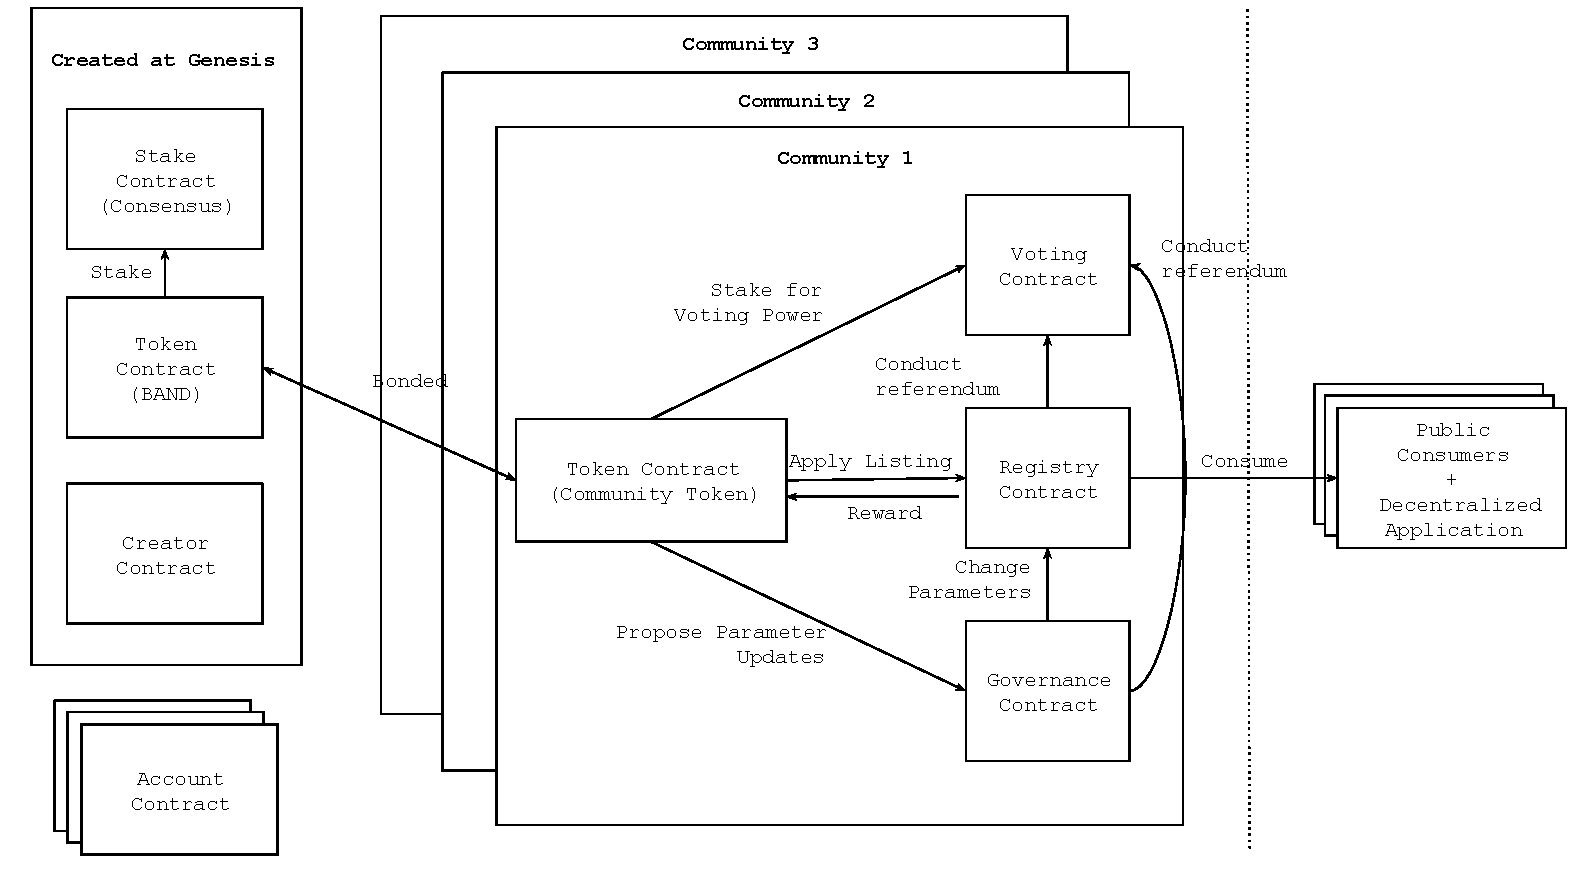
\includegraphics[width=\textwidth]{tcr}
	\captionsetup{labelformat=empty}
    \caption{Overview of the interactions between smart contracts necessary to enable Band TCR protocol.}
    \label{fig:tcr}
\end{figure}

\paragraph{Voting Contract} implements Partial-Lock Commit-Reveal Voting data structure~\cite{plcrvoting}. The contract is binded with one token contract and allows anyone to transfer their token into it. Once a Voting contract is created, a Registry contract can request it to create a poll to resolve a proposal challenge. Note that a Voting contract allows a user to participate in multiple polls concurrently while still enforces that each user has voting power proportional to the number of staked tokens.

\paragraph{Registry Contract} implements the core functionality of the TCR by maintaining a list of curated data on the blockchain. The contract is binded with one Voting contract and one Governance contract at the contract initialization. It allows a user to submit and/or challenge a proposal and appropriately distribute the rewards after the conflict is resolved. The contract’s parameters are set to the default values at initialization, but can be changed in a decentralized manner through its Governance contract.

\paragraph{Governance Contract} is a specialized Registry contract designed for governing  the parameters of another Registry contract (so called the target). In this contract, a proposal is a packed binary representation of the target's parameters. If the proposal is approved (i.e. not getting challenged down), the parameter change is applied to the target. Note that due to the high impact nature of the proposals on this contract, {\tt min\_stake} and {\tt pending\_duration} should be set to reasonably high values to disincentivize attackers.

\subsection{Plasma: Data Curation at Scale with Privacy} \label{sec:permissioned-community}
In addition to the public platform, Band protocol supports permissioned token-curated registry. In this model, curated data is not directly available on the Band public main chain but instead live on another blockchain so called a side-chain. There are two major benefits of this side-chain blockchain structure:

\begin{itemize}
\setlength\itemsep{0em}
\item Side-chain can be configured to either be permissioned or permissionless. Permissioned chain allows the set of pre-specified validators to have total control over data publicity and privacy. Permissionless chain behaves similarly to the Band chain, but with its own set of governing rules and validators.
\item Running TCR protocol and keeping curated data in the side chain reduces the workload on the main chain. Therefore, Band ecosystem is able to scale horizontally and handle more than a million transactions per second, spread among all the side chains without compromising the blockchain security.
\end{itemize}

\subsubsection{On-Chain Architecture}
Band protocol side-chain architecture closely resembles Ethereum’s proposed Plasma framework~\cite{poon2017plasma}. On the main Band chain, anyone can create a Plasma contract that is binded to a Token contract. The following is a quick summary of protocol.

\begin{figure}[ht!]
    \centering
    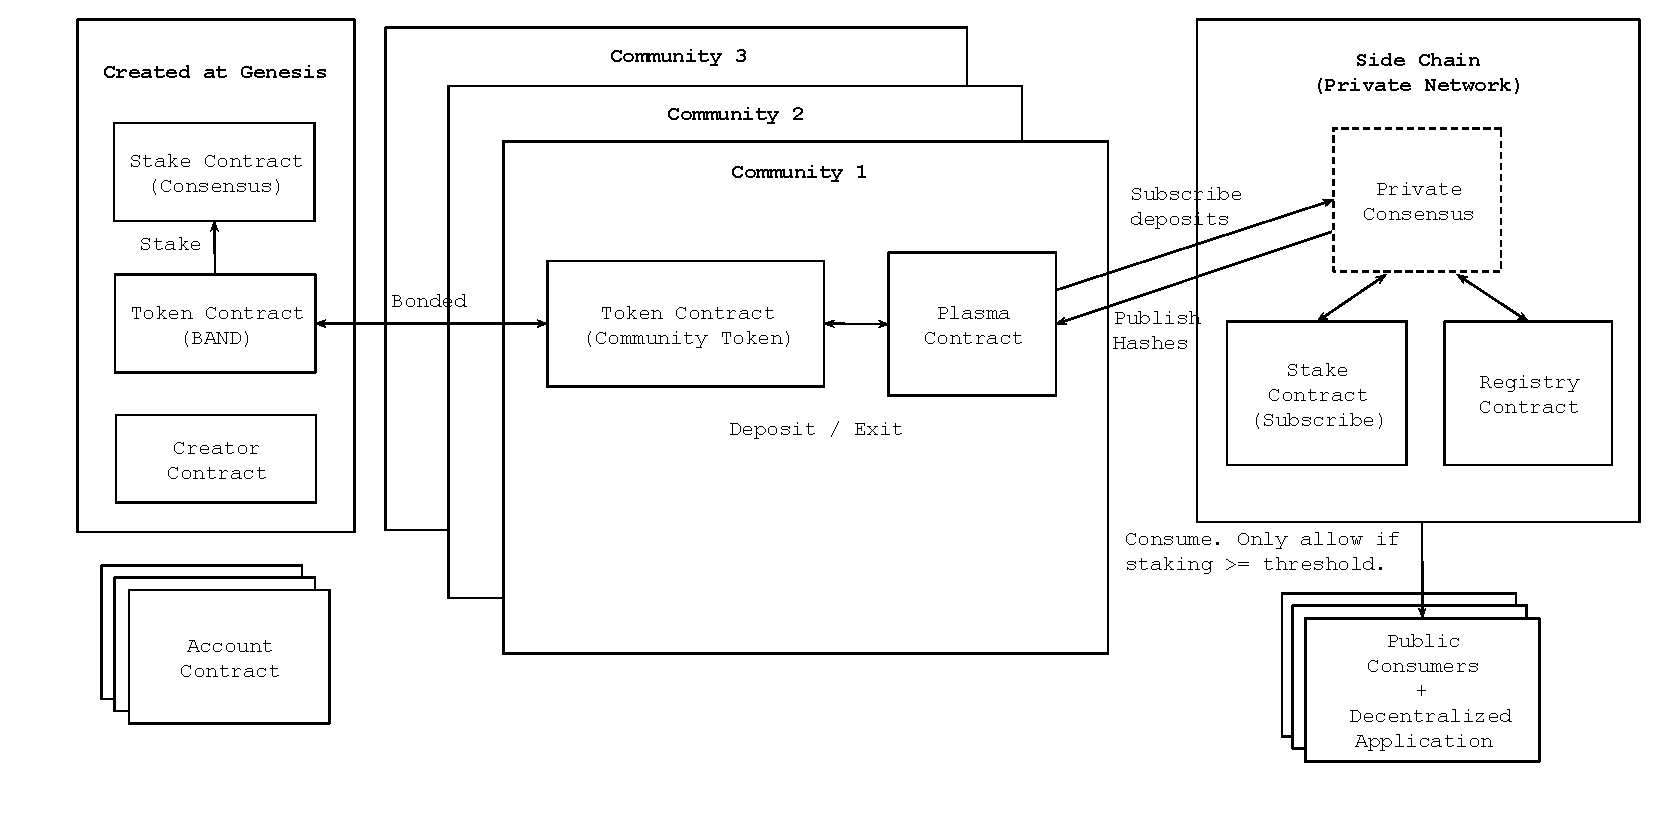
\includegraphics[width=\textwidth]{plasma}
	\captionsetup{labelformat=empty}
    \caption{Overview of the interactions between smart contracts and between main-chain and side-chain in the use case of permissioned TCR. Data is curated by a private consortium. Members can access the data if they stake enough tokens (i.e. subscribe).}
    \label{fig:plasma}
\end{figure}

\begin{enumerate}
\setlength\itemsep{0em}
\item Plasma contract is created on the main chain, and a side-chain is spun up to synchronize with the Plasma contract. The synchronization includes: (1) publishing the hash of all the blocks on the side-chain, and (2) updating the side-chain state to reflect new blocks that the Plasma contract produces as a result of a user transfers tokens in.
\item A user may transfer tokens to the Plasma contract. This transfer will appear as a block on the series of hashes that the contract maintains.
\item If a user would like to exit the side-chain (i.e. Plasma exit) either because of the need to cash out or because of any malicious actions, he or she can submit Plasma exit transaction with the proof that the transaction exists in one of the block hashes.
\item The exit transaction will be pending for a challenging period (default to 1 day), during which anyone can challenge the exit by submitting the proof that the transaction has already been spent in one of the subsequent block hashes.
\item If there is no successful challenge during the challenging period, the withdrawal is successful and the Plasma contract transfers fund to user on the main chain. If a challenge is successful, the staked tokens are awarded to the challenger, and the exit transaction fails.
\item Exit transactions are prioritized by block number at which the transaction is in. This allows members to still Plasma exit in the case where the validator submits a bogus transaction saying that he or she is the owner of all the funds and withdraw immediately.
\end{enumerate}

\paragraph{Plasma Contract} keeps track of the side-chain application states in the form of a series of block hashes. Band Protocol's Plasma contract is initially designed to follow the community-reviewed specification of Plasma MVP provided by the Ethereum community and OmiseGO team~\cite{plasmamvp1,plasmamvp2} , but in Band native contract format. It is responsible for accepting new tokens into the side-chain, and resolving Plasma exit. It allows the validators to publish new block hashes, and allows other members to transfer funds in, withdraw funds out, and challenge another person’s withdrawal. 

\paragraph{Side-chain Implementation} The Band chain distribution can be configured to run in side-chain mode by providing the remote chain address and the Plasma contract address. Under this mode, the blockchain will broadcast the hash of every block produced on the side-chain as one transaction to the main chain. It will also subscribe to the main chain update so that new token transfers to the Plasma contract are constantly reflected on the side-chain.  

\subsection{Upgradability} \label{sec:other-applications}
Immutability of smart contracts, while has it pluses, also poses a major challenge to the blockchain community. In particular, non-upgradable smart contracts cannot have security fixes easily once deployed. With Band protocol, there are two different schemes that Band chain can solve this problem.

\paragraph{On-Chain Upgrade} In Band protocol, any function on a smart contract can be encoded to and decoded from a wire format binary data. A TCR-like contract can be created to allow members to vote on any arbitrary binary data for a specific target contract. Once approved, this binary data can be interpreted to the target contract's C++ function call, which can then be called to upgrade the contract arbitrarily through a provided interface (which can be as arbitrary as taking a function implementation and overwriting another existing function with it).

\paragraph{Blockchain-Level Smart Contract}
Because smart contracts on the Band chain are community curated, built, and run on the same layer as the blockchain source code itself. In order to make sure that the decision to upgrade is unanimous, voting based on Band token should be performed (See~\cref{subsubsec:govern}). If a fix or upgrade is agreed, such implementation can be made directly through the blockchain source code. Note that this scheme relies on block validators picking up the changes. Due to the high stake in block reward, the validators are incentivized to pick up changes quickly, or else people will stop delegating Band tokens for them. 

\subsection{Attack Vectors} \label{sec:attack-vector}
This section describes possible attack vectors to Band chain, and plans to mitigate the potential problems.

\subsubsection{Community Token Price Manipulation}
\paragraph{Concern:} Due to the predictable nature of the price of community tokens, it is possible that malicious actors can manipulate the price of the tokens in their favor. For instance, if the attackers notice there is a buy transaction broadcasted to the network, they expect the price to move up, and thus buy the tokens themselves before the price rises (i.e. Front-Running~\cite{pagano1993front}).

\paragraph{Mitigation:}

\begin{itemize}
\setlength\itemsep{0em}
\item Every buy and sell transaction includes the limit price at which the transaction sender is willing to buy or sell. If the price moves beyond the limit price, the transaction is voided, and the sender is protected from the rapid price movement.
\item There is no concept of transaction fees in Band chain, which means all transactions have the same priority. Front-running is not possible unless the attackers are one of the block validators. Block validators hold large amount of tokens in the system and have very strong economic disincentive to attack Band chain.
\item Community token creators are encouraged to set price spread when defining the token’s bonding curve. That way, making profits from buying and quickly selling becomes much more difficult.
\end{itemize}

\subsubsection{Replay Attack}
\paragraph{Concern:} Malicious validators and transaction propagators can save or withhold a transaction and replay it later when the transaction is in their favor. For example, if a user submit a transaction to transfer tokens to the validators, the validators may replay that transaction again to receive more tokens.

\paragraph{Mitigation:} Every transaction must contain a nonce. The preloaded Account contract provided with the blockchain layer contains a nonce. In order for the Account contract to approve and delegate a transaction, not only does the signature needs to match, the nonce must be strictly greater than the nonce of the previous transaction approved by this Account contract.

\subsubsection{Denial of Service (DOS)}
\paragraph{Concern:} Malicious actors may spam the blockchain with meaningless transactions to clog the network. Thus, valid transactions will not be processed in a timely manner.

\paragraph{Mitigation:} It will take a huge amount of Band to remotely affect the blockchain bandwidth. For instance, in order to consume 30\% of network capacity, the attackers must possess 30\% of Band total supply. It is likely not economically favorable for people to own so much stake in Band to attack the system themselves.

\subsubsection{Attacks on the Consensus Level}
\paragraph{Concern:}
Is Tendermint secured against well-known blockchain possible vulnerabilities, including but not limited to long-range attack, censorship attack, and fork accountability?

\paragraph{Mitigation:}
Band chain chooses to build the blockchain infrastructure based off the Tendermint platform due to their well-known adoptions in the blockchain community. Most of the possible attack vectors on the consensus level have been discussed in the Cosmos white paper and Tendermint supporting academic theses~\cite{cosmoswhitepaper,buchman2016tendermint,kwon2014tendermint}.

\subsubsection{Wealthy Attacker}
\paragraph{Concern:} Wealthy adversary may use large amount of capital to buy tokens and obtain the majority vote, essentially conduct a 51 percent attack on the registry.  

\paragraph{Mitigation:} Our proposed solution to create one token per registry which links the value of token directly with the quality of the data can mitigate the problem. If such attack occurs and data becomes less useful for the users, the value of token is essentially destroyed since no more followers and applicants will wish to buy tokens and submit data. Our protocol is similar to Casper proposed by Ethereum community -- such attacker will incur so large financial loss that it does not make economic sense to attack a registry. Each community can also decide to fork to another registry, rendering the attack pointless. 


\bibliographystyle{unsrt}
\bibliography{paper}

\end{document}

